%%
% このファイルは、筑波大学情報学群情報メディア創成学類の
% 卒業研究論文本体のサンプルです。
% このファイルを書き換えて、この例と同じような書式の論文本体を
% LaTeXを使って作成することができます。
% 
% PC環境や、LaTeX環境の設定によっては漢字コードや改行コードを
% 変更する必要があります。
%%
\documentclass[a4paper,11pt]{jreport}

%%【PostScript, JPEG, PNG等の画像の貼り込み】
%% 利用するパッケージを選んでコメントアウトしてください。
%\usepackage{graphicx} % for 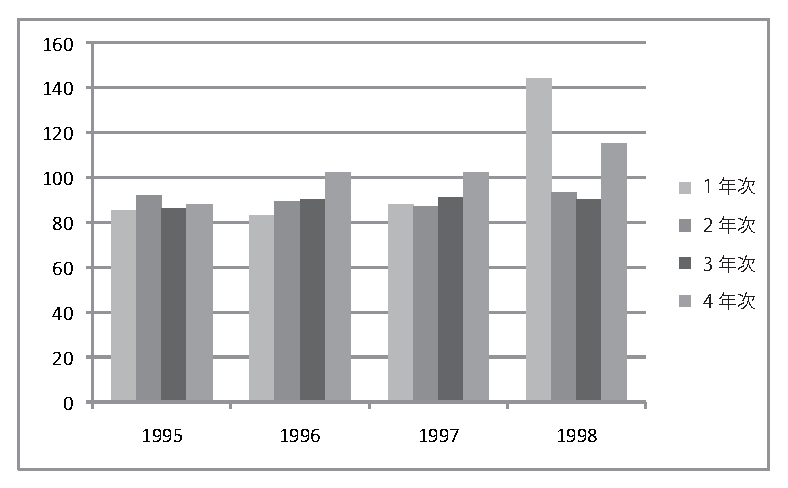
\includegraphics[width=3cm]{sample.eps}
\usepackage{epsfig} % for 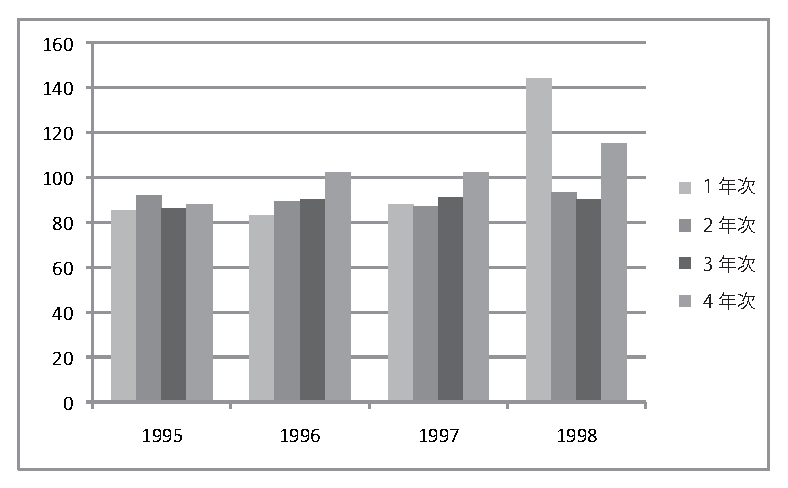
\psfig{file=sample.eps,width=3cm}
%\usepackage{epsf} % for \epsfile{file=sample.eps,scale=0.6}
%\usepackage{epsbox} % for \epsfile{file=sample.eps,scale=0.6}

\usepackage{times} % use Times Font instead of Computer Modern

%%%%%%%%%%追加
\usepackage{amsmath,amsthm,amssymb,cases}
\usepackage{algorithmic,algorithm}

\setcounter{tocdepth}{3}
\setcounter{page}{-1}

\setlength{\oddsidemargin}{0.1in}
\setlength{\evensidemargin}{0.1in} 
\setlength{\topmargin}{0in}
\setlength{\textwidth}{6in} 
%\setlength{\textheight}{10.1in}
\setlength{\parskip}{0em}
\setlength{\topsep}{0em}

%\newcommand{\zu}[1]{{\gt \bf 図\ref{#1}}}

%% タイトル生成用パッケージ(重要)
\usepackage{mast-jp-utf8}

%% タイトル
%% 【注意】タイトルの最後に\\ を入れるとエラーになります
\title{クエリ依存型リンク解析手法における\\スコア近似に関する研究}
%% 著者
\author{佐藤 豪}
%% 指導教員
\advisor{古瀬 一隆 陳 漢雄}

%% 年月 (提出年月)
%% 年月は必要に応じて書き替えてください。
\majorfield{ } \yearandmonth{2016年 1月}



\begin{document}
\maketitle
\thispagestyle{empty}
\newpage

\thispagestyle{empty}
\vspace*{20pt plus 1fil}
\parindent=1zw
\noindent
%%
%% 論文の概要(Abstract)
%%
\begin{center}
{\bf 概要}
\vspace{5mm}
\end{center}
私たちが普段使用しているWEBページの検索エンジンに用いられている手法の1つに、
リンク構造に基づいて得点を与えるSALSAアルゴリズムがある。
SALSAアルゴリズムはクエリ依存型のリンク解析手法であり、よりクエリに適した検索結果を得ることができる。一方で、クエリが与えられてからWEBグラフの抽出を行いリンク構造を取得し、各ページのスコア計算を行うため多くの応答時間がかかってしまう。

先行研究では、SALSAアルゴリズムの一部をクエリが与えられる前に処理することで高速化を図る手法が提案された。従来のSALSAアルゴリズムに比べて高速化することに成功したものの、ランキング精度においては著しく低い結果となり、クエリに適した検索結果が得られるというクエリ依存型リンク解析手法の長所が失われてしまった。そこで、本論文では先行研究の手法を改善し、ランキング精度を保ちつつ、高速化を行う手法を提案する。

本研究では、クエリ依存型リンク解析手法SALSAにおいて、クエリに適した検索結果が得られるという長所を保ちつつ、検索の高速化を行うことを目的とする。

%%%%%
\par
\vspace{0pt plus 1fil}
\newpage

\pagenumbering{roman} % I, II, III, IV 
\tableofcontents
\listoffigures
%\listoftables

\pagebreak \setcounter{page}{1}
\pagenumbering{arabic} % 1,2,3


%%%%%%%%%%%%%%%%%%%%%%%%%%%%%%%%%%%%%%%%%%%%%%%%
\chapter{序論}

世界中に10億件以上存在するWEBサイトの中から、必要な情報を手探りで探すことは困難である。
そのような場合、検索エンジンを用いることが有効である。検索エンジンは、ユーザーが必要とする情報に関連した検索キーワードを受け取り、そのキーワードに関連するWEBページの集合を抽出し、検索結果としてユーザーに掲示する。検索結果として掲示されるWEBページの集合は、検索キーワードとの関連度が高く、ユーザーにとって役に立つWEBページが上位に表示されることが望ましい。このように、ある検索ワードに関連するWEBページの集合に対して、ユーザーに掲示するための順位付けを行う手法をWEBランキングアルゴリズムと呼ぶ。

WEBランキングアルゴリズムは大きく分けて2種類ある。1つ目は、WEBページのテキストやHTML構造を解析することで内容得点を計算し、順位付けを行う手法である、2つ目は、WEBページ間のリンク構造に基づいてスコア計算を行い、順位付けを行うリンク解析手法である。本論文では後者のリンク解析手法を扱うものとする。

リンク解析手法のアルゴリズムで有名なものとしてPageRankアルゴリズムやHITSアルゴリズムが挙げられる。さらに近年の研究では、PageRankアルゴリズムとHITSアルゴリズムの長所を取り入れたSALSAアルゴリズムと呼ばれるリンク解析手法が、ランキング精度において他のWEBランキングアルゴリズムより優れているという報告がされている。

PageRankアルゴリズムは、検索キーワードに依存せずスコア計算を行い、順位付けをすることができる。このようなリンク解析手法をクエリ独立型と呼ぶ。一方でHITSアルゴリズムやSALSAアルゴリズムは、検索キーワードが与えられてからスコア計算と順位付けを行う。このようなリンク解析手法をクエリ依存型と呼ぶ。したがって、これらのアルゴリズムを検索エンジンで用いる場合、検索キーワードが与えられる前にスコア計算を行うPageRankアルゴリズムは高速に応答することができるのに対し、検索キーワードが与えられてからスコア計算を行うHITSアルゴリズムやSALSAアルゴリズムは応答時に無視できないほどの時間がかかってしまう。

この問題の解決策として、クエリ依存型リンク解析手法において時間のかかるスコア計算を前処理化することで、応答時間を減らすという手法が過去に提案された。これらの手法では、検索キーワードが与えられる前にあらかじめWEBページのクラスタリングを行い、クラスタ内での各ページのスコア計算を行う。検索キーワードが与えられた後は、そのクラスタとスコアを用いて結果を近似し、WEBランキングを作成する。しかし、これらの手法では近似したスコアと本来のSALSAアルゴリズムによるスコアが大きく異るため、応答時間は早くなるがランキング精度が下がる結果となった。

そこで本研究では、クエリ依存型リンク解析手法SALSAの前処理化におけるクラスタリングとスコア近似を改善することで、従来のSALSAアルゴリズムにより近いWEBランキングを作成することができ、かつ応答時間の少ない手法を提案する。



%%%%%%%%%%%%%%%%%%%%%%%%%%%%%%%%%%%%%%%%%%%%%%%%
\chapter{関連研究}

本章では、クエリ依存型リンク解析手法SALSAに関する技術について、特に関連のある研究について紹介する。

\section{WEBランキングアルゴリズムの歴史}

巨大化したWEBの中から目的のWEBページを見つけるには、検索エンジンを使うのが有効である。検索エンジンに与えた検索キーワード、別名クエリと関連のあるページに対して順位付けをするのがWEBランキングアルゴリズムである。

1998年までWEBランキングアルゴリズムは、WEBページのテキストやHTML構造といった内容得点で順位付けを行っていた。この内容得点というのは、各WEBページにどこにどれほどクエリの文字列が含まれているのか計算したものであった。しかし、WEBが巨大化し限りなく増大していったことや、内容得点がスパムの影響を受けやすかったことから、1998年までには従来の内容得点は有効でないことが明らかになっていた。

そこで、内容得点だけではなく、WEBのハイパーリンク構造に対して有向グラフを作成し、その有向グラフを用いてWEBページの人気得点を計算するリンク解析手法が登場した。

\begin{figure}[htbp]
\begin{center}
%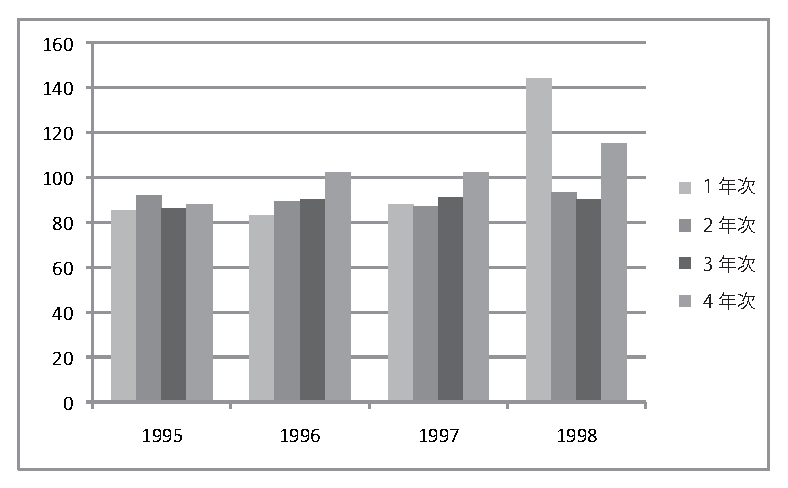
\includegraphics[width=3cm]{sample.eps}
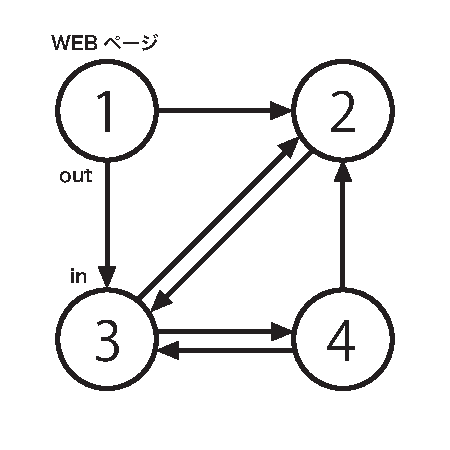
\psfig{file=image/webgraph.eps,scale=0.8}
%\epsfile{file=sample.eps,scale=0.6}
\end{center}
\caption{WEBグラフ}
\label{figure:sample}
\end{figure}

これによって従来の内容得点によるランキングよりも品質が向上し、検索エンジンの利用者は劇的に増え、リンク解析手法はWEBランキングアルゴリズムの主流となった。


\section{PageRank}

PageRankは、当時Stanford Universityに在学していたSergey BrinとLarry Pageの2人の計算機科学科の学生によって開発されたものであり、開発者の名前がアルゴリズムの由来となっている。これがのちのWEB検索エンジンGoogleであり、このアルゴリズムの基本的な概念は「多くの良質なページからリンクされているページは、 やはり良質なページである」 という再帰的な関係をもとに、全てのページの重要度を判定したものである。

以下の図2.2はPageRankの概念図である。あるページのスコアを、そのページに存在する出リンク数で割った数が、それぞれの被リンク先のスコアに加算されるという関係になっている。

\begin{figure}[htbp]
\begin{center}
%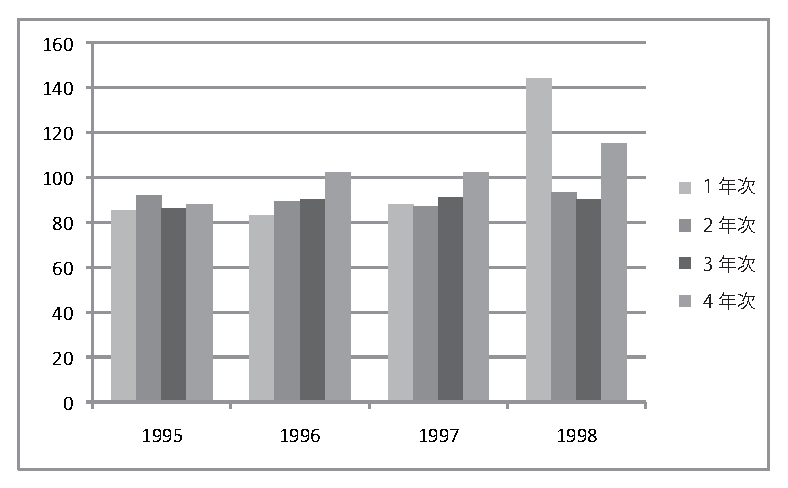
\includegraphics[width=3cm]{sample.eps}
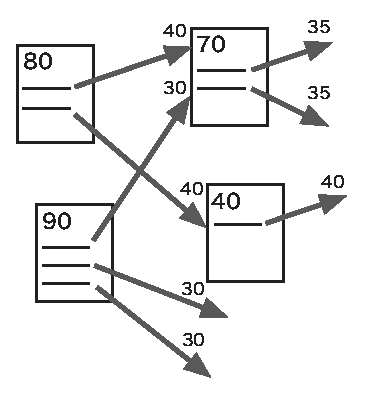
\psfig{file=image/pagerank.eps,scale=1.0}
%\epsfile{file=sample.eps,scale=0.6}
\end{center}
\caption{PageRankの概念図}
\label{figure:sample}
\end{figure}

PageRankは、WEBグラフにランダムウォークモデルを適応し、各ページヘの遷移確率によってWEBランキングを作成する。あるページからそのページが指している全リンク先へとランダムに遷移する確率と全てのWEBページへとランダムに遷移する確率を足したスコアがPageRankのスコアになる。

PageRankのスコア計算は以下の式(2.1)で定義される。

\begin{equation}
\pi^T = \pi^T(\alpha S + (1 - \alpha)E) 
\end{equation}

ここで$\pi^T$はPageRankベクトルであり、$\alpha$は0.85程度のスカラー値であり、行列$S$はページ$i$から
そのリンク先であるページ$j$への遷移確率行列である。また行列$E$は全てのWEBページヘのレポーテーション行列である。

ここで行列$S$は、ページ$i$からそのリンク先ページ$j$への遷移確率を示すので以下のように定義することができる。

\begin{equation}
S_(i,j) =
\begin{cases}
\; 1/out(i) (out(i)はノードiの出リンク数) \\
\; 0 (ノードiからノードjへのリンクがないとき)
\end{cases}
\end{equation}

また、行列$E$はページ$i$から全てのページへのランダムな遷移を示すので、以下(2.3)のように定義することができる。

\begin{equation}
E_(i,j) = 1
\end{equation}

PageRankの特徴の1つとして、クエリ独立型のリンク解析手法であるという点が挙げられる。
これは、クエリに関係なく、最初から全てのWEBページに対するWEBランキングが決定しているということである。クエリが与えられてからは、既に作成されているWEBランキングに適切なフィルタリングを施し、検索結果としてWEBランキングを表示するだけである。このためPageRankは、HITSやSALSAのようなクエリ依存型のリンク解析手法に比べ、応答時間が短い。

\section{HITS}

HITSは、1998年にJon Kleinbergによって発明された。PageRankと同様、WEBページに関連した人気得点を作るのにWEBのハイパーリンク構造を用いる。しかし、PageRankと違いHITSは各ページに対して権威スコアとハブスコアという2種類のスコアを作成し、権威ページとハブページを定義する。

権威ページはたくさんの入リンクを持つページであり、ハブはたくさんの出リンクを持つページである。
また、良い権威ページたちは良いハブページたちによってリンクされており、良いハブページたちは良い権威ページたちをリンクしているという循環的な性質を持っている。

\begin{figure}[htbp]
\begin{center}
%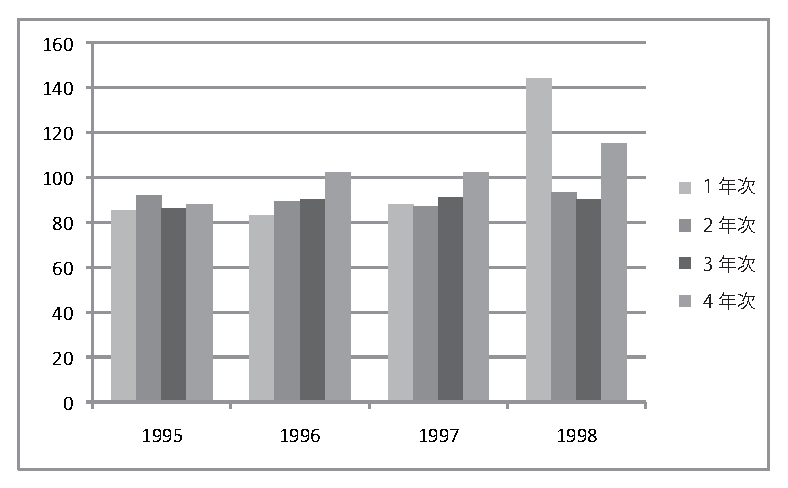
\includegraphics[width=3cm]{sample.eps}
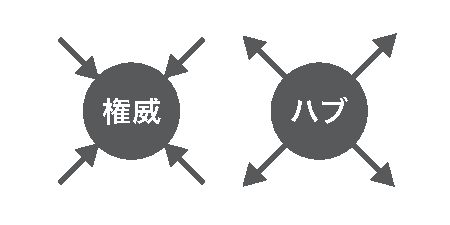
\psfig{file=image/hits.eps,scale=1.0}
%\epsfile{file=sample.eps,scale=0.6}
\end{center}
\caption{権威とハブ}
\label{figure:sample}
\end{figure}

HITSではWEBの構造を有向グラフとして捉え、各スコアの計算を行う。権威スコアとハブスコアを
計算する上で有向グラフの隣接行列$L$を用いて以下のように行列の形で書くことができる。

\begin{equation}
L_(i,j) =
\begin{cases}
\; 1 (ノードiからノードjへのリンクがあるとき) \\
\; 0 (ノードiからノードjへのリンクがないとき)
\end{cases}
\end{equation}

この隣接行列$L$を用いて、権威スコア$x$とハブスコア$y$の計算は以下の式(2.5)(2.6)(2.7)で定義される。
この計算は、ハブスコアの初期値を$y^(0) = e$とし、各スコアが収束するまで計算を繰り返す。ここで$e$は全て1の列ベクトルである。

\begin{eqnarray}
x^{(k)} = L^Ty^{(k-1)} \\
y^{(k)} = Lx^{(k)} \\
k = k + 1
\end{eqnarray}

HITSの特徴の一つとして、クエリ依存型のリンク解析手法であるという点が挙げれられる。クエリが与えられると、クエリに関連するページの集合であるroot setの抽出を行う。そこから、root setとリンク関係にある距離1のページを含めた集合であるbase setに拡張する。その後、base setの隣接行列を作成し、base set内の各ページに対してスコアを割り当て正規化を行い、WEBランキングを作成する。以下の図2.4はroot setからbase setを作成する処理を視覚化したものである。

\begin{figure}[htbp]
\begin{center}
%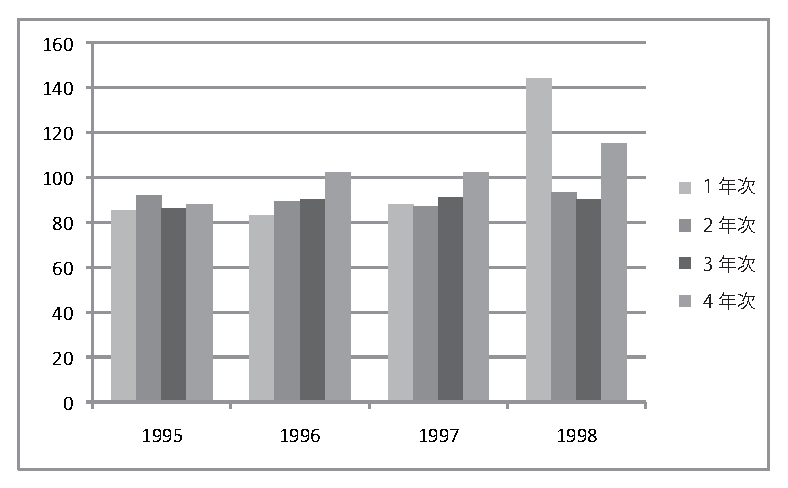
\includegraphics[width=3cm]{sample.eps}
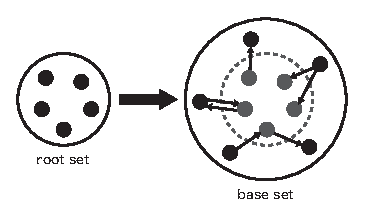
\psfig{file=image/hits2.eps,scale=1.0}
%\epsfile{file=sample.eps,scale=0.6}
\end{center}
\caption{root setとbase set}
\label{figure:sample}
\end{figure}

HITSはクエリに適した検索結果を得られるが、クエリが与えられてからbase setの作成とスコア計算を行うため、無視できないほどの応答時間がかかってしまう。

さらに、ランキングの対象となるbase setをWEBのリンク構造から作成するため、クエリと関係の小さいページがランキング上位に表示されてしまうことがある。この現象を話題の横滑り(topic draft)と呼ぶ。

\section{SALSA}

SALSAは、2000年にRonny LampelとShlomo Moranによって発明された。クエリ依存型のリンク解析手法の一つで、PageRankとSALSAの長所が組み込まれている。HITSと同じように、SALSAはWEBページの権威得点とハブ得点の両方を作り、PageRankのように、それらはマルコフ連鎖から作られる。そのため、近年の研究においてSALSAはPageRankやHITSよりも、さらにクエリに適した検索結果が得られるということがわかっている。

SALSAでは、HITSで用いた隣接行列$L$に対し、各ノードの出リンク数および入リンク数によって行と列の両方の重み付けを用いている。これは、HITSにおける話題の横滑り現象を回避するためである。$L$の各非ゼロ行列をその行の総和で割ったものを$L_r$、$L$の各非ゼロ行列をその列の総和で割ったものを$L_c$とし、これらは以下のように定義される。

\begin{equation}
L_{r(i,j)} =
\begin{cases}
\; 1/out(i) (out(i)はノードiの出リンク数) \\
\; 0 (ノードiからノードjへのリンクがないとき)
\end{cases}
\end{equation}

\begin{equation}
L_{c(i,j)} =
\begin{cases}
\; 1/in(i) (in(i)はノードiの入リンク数) \\
\; 0 (ノードiからノードjへのリンクがないとき)
\end{cases}
\end{equation}

権威スコア$x$とハブスコア$y$の計算は以下の式(2.10)(2.11)(2.12)で定義される。
HITSと同様に、ハブスコアの初期値を$y^(0) = e$とし、各スコアが収束するまで計算を繰り返す。

\begin{eqnarray}
x^{(k)} = L_c^Ty^{(k-1)} \\
y^{(k)} = L_rx^{(k)} \\
k = k + 1
\end{eqnarray}

SALSAもHITSと同様に、クエリが与えられてからbase setの作成とスコア計算を行うため、無視できないほどの応答時間がかかってしまう。

%%%%%%%%%%%%%%%%%%%%%%%%%%%%%%%%%%%%%%%%%%%%%%%%
\chapter{提案手法}

本章では、クエリ依存型リンク解析手法であるSALSAアルゴリズムを高速化する手法について解説する。

\section{クエリ依存型リンク解析手法高速化の概要}

以下の図3.1はPageRankに代表されるクエリ独立型リンク解析手法における処理の流れを視覚化したものである。

\begin{figure}[htbp]
\begin{center}
%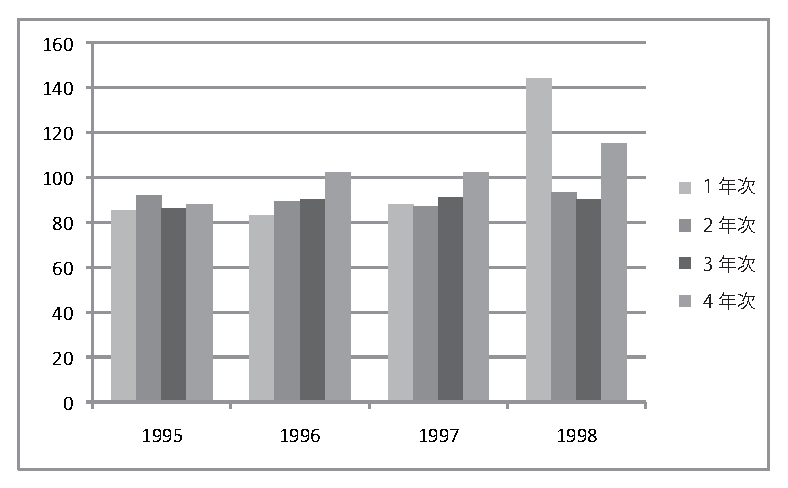
\includegraphics[width=3cm]{sample.eps}
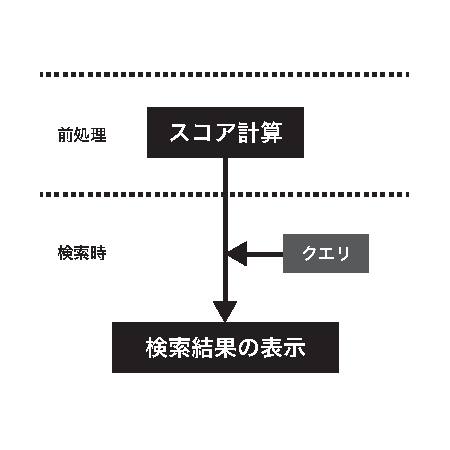
\psfig{file=image/query.eps,scale=1.0}
%\epsfile{file=sample.eps,scale=0.6}
\end{center}
\caption{クエリ独立型リンク解析手法}
\label{figure:sample}
\end{figure}

クエリ独立型リンク解析手法では、あらかじめ全WEBページのスコアを計算し、クエリに依存することなくWEBランキングを作成する。クエリが与えられてからは適切なフィルタリングを施しランキングを表示するだけなので、応答時間は極めて短い。

以下の図3.2はクエリ依存型リンク解析手法における処理の流れを視覚化したものである。クエリ依存型リンク解析手法では、WEBページの集合からクエリに関連する部分をbase setとして抽出し、抽出されたWEBページの権威スコア、ハブスコアを計算し、ランキングを表示する。クエリが与えられてからbase setの作成、各スコアの計算を行うため長い応答時間がかかってしまう。

そこで、先行研究では、WEBグラフの抽出と各スコアの計算を前処理化することでクエリが与えられてからのランキング作成を高速化する手法が提案された。この手法では、あらかじめWEBグラフをクラスタリングしておき、各クラスタ内でのWEBページに対して権威スコアとハブスコアを計算しておく。その後、クエリが与えられるとクエリに関連するWEBページを含むクラスタを抽出し、そこからクラスタ内での各WEBページのスコアを元に最終的なスコアを近似する。

\begin{figure}[htbp]
\begin{center}
%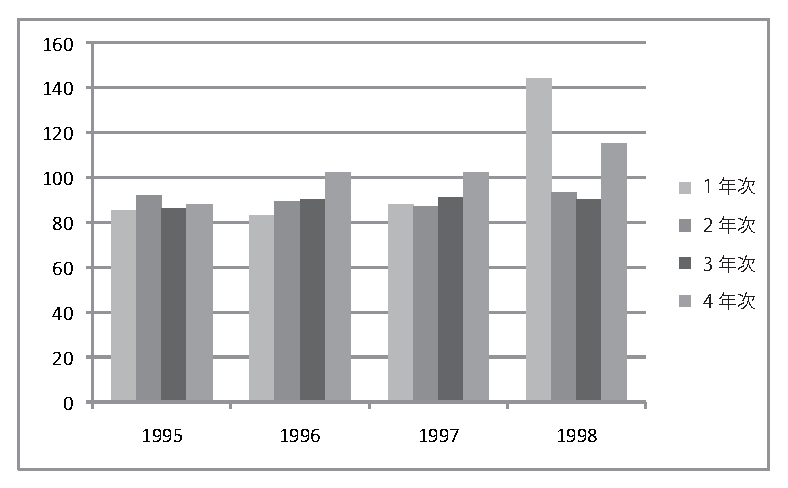
\includegraphics[width=3cm]{sample.eps}
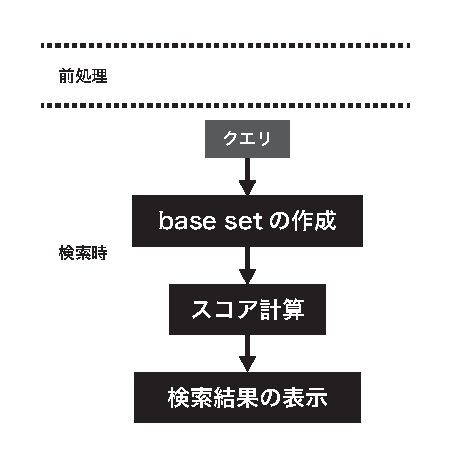
\psfig{file=image/query2.eps,scale=1.0}
%\epsfile{file=sample.eps,scale=0.6}
\end{center}
\caption{クエリ依存型リンク解析手法}
\label{figure:sample}
\end{figure}

以下の図3.3は高速化したクエリ依存型リンク解析手法における処理の流れを視覚化したものである。
図の左側は従来のアルゴリズムによる処理を示し、右側は高速化したアルゴリズムによる処理を示している。

\begin{figure}[htbp]
\begin{center}
%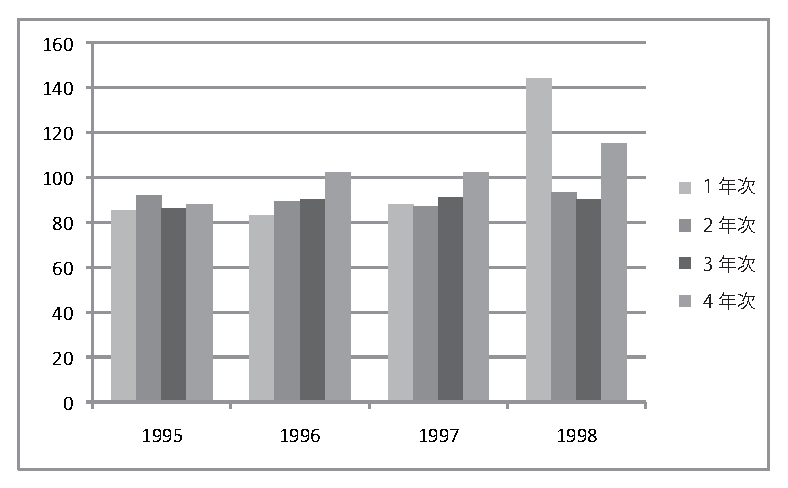
\includegraphics[width=3cm]{sample.eps}
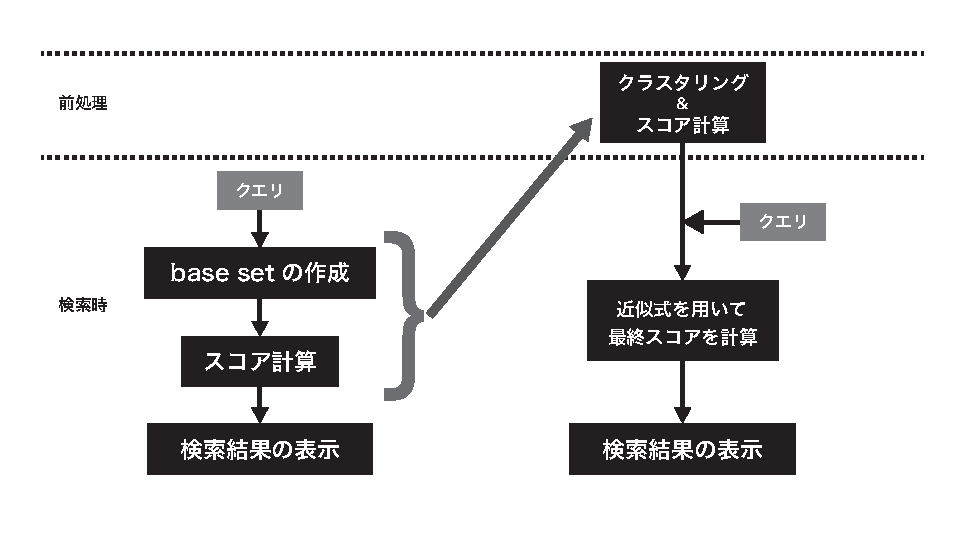
\psfig{file=image/query3.eps,scale=1.0}
%\epsfile{file=sample.eps,scale=0.6}
\end{center}
\caption{クエリ依存型リンク解析手法の高速化}
\label{figure:sample}
\end{figure}

全てのWEBページをクラスタリングし、各スコアの計算をあらかじめ処理しておくことで、クエリが与えられてからの応答時間を大幅に短くすることができる。しかし、高速化した手法で求めたWEBランキングと、従来の方法で求めたWEBランキングには大きな差ができてしまった。これは、適切なクラスタリングが行われず、最終的なスコア近似の精度が低くなり、クエリと関連の少ないページがランキングに入ってしまうためであると考えられる。

\newpage

\section{提案手法の概要}

この節では、まずはじめに提案手法の概要について解説する。高速化したSALSAアルゴリズムでは、従来のSALSAアルゴリズムより高速な処理が可能だが、従来のSALSAアルゴリズムで作成したランキングと比べてランキングの精度が落ちてしまうという問題があった。そこで本研究では、従来のSALSAアルゴリズムより高速で、かつ従来のSALSAアルゴリズムに近いWEBランキングを作成する手法を提案する。具体的には、先行研究と同様にWEBページのクラスタリングと各スコアの計算を前処理として行うが、そのクラスタリング部分と最終スコアの近似部分において改良を加える。

クラスタリングでは、まず少数のページで初期セットを作成し、そこにリンク関係のあるページを追加していくことでクラスタを大きくしていく。先行研究による高速化アルゴリズムでは、初期セットのサイズを固定し、全てのページが1つ以上のクラスタに所属するまでクラスタリングを行う。この場合、最終スコアの近似を行う際に、多くのクラスタに所属しているページほどスコアが大きくなり、適切なランキングを得ることができない。

\begin{figure}[htbp]
\begin{center}
%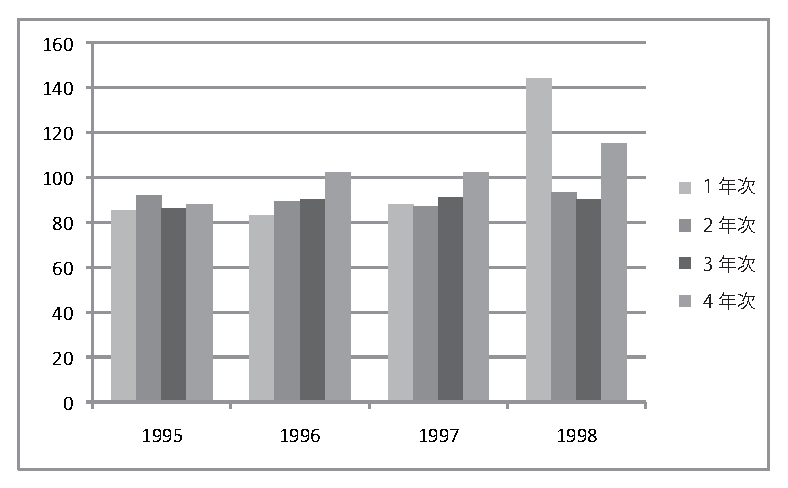
\includegraphics[width=3cm]{sample.eps}
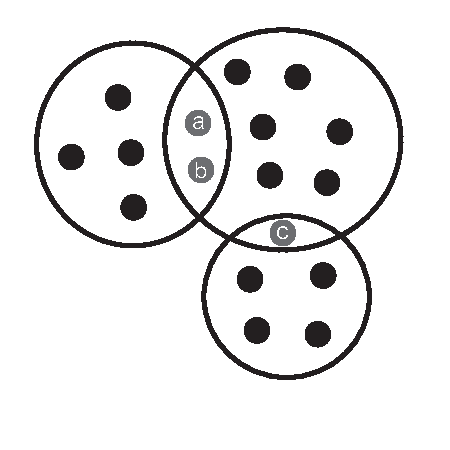
\psfig{file=image/clustering1.eps,scale=1.0}
%\epsfile{file=sample.eps,scale=0.6}
\end{center}
\caption{全てのページが1つ以上のクラスタに所属}
\label{figure:sample}
\end{figure}

そこで今回提案する手法では、全てのページはそれぞれ1つのクラスタにのみ所属するものとする。したがって、1度クラスタに追加されたページが再び別のクラスタに所属することはないので、クラスタリングにおける処理の高速化も期待することができる。これに伴い、最終スコアの近似式に改良を加える。

\begin{figure}[htbp]
\begin{center}
%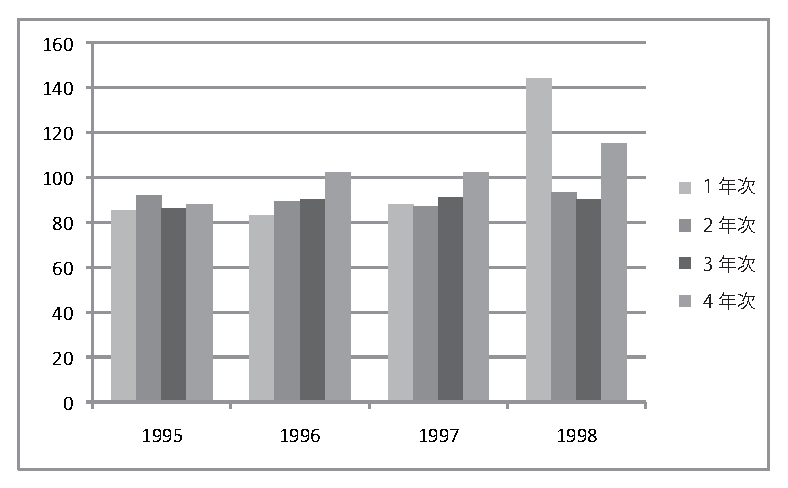
\includegraphics[width=3cm]{sample.eps}
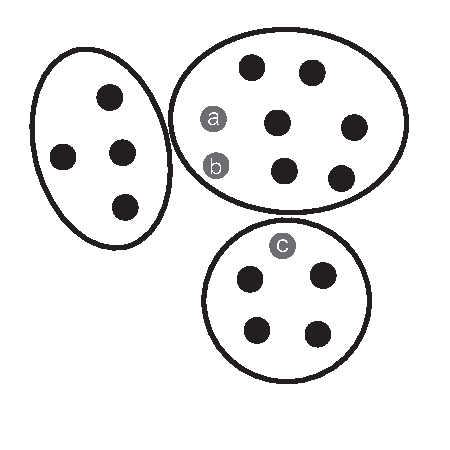
\psfig{file=image/clustering2.eps,scale=1.0}
%\epsfile{file=sample.eps,scale=0.6}
\end{center}
\caption{全てのページが1つのクラスタに所属}
\label{figure:sample}
\end{figure}

詳しいクラスタリングアルゴリズム、スコアの近似については、次節以降で解説する。

\section{クラスタリングアルゴリズム}

高速化のための前処理として、全てのWEBページをクラスタと呼ばれる集合に分けて、それぞれのクラスタ内で各スコア計算を行う。ここでは、クラスタリングアルゴリズムについて解説する。

まず、クラスタのseed pageを選択する。seed pageは、まだどのクラスタにも属していないページのうち、出リンク数、入リンク数の多いものを選択する。

その後、seed pageと相互リンクしているページ、出リンク先や入リンク元となるページを順にクラスタへ追加し、初期セットを作成する。以下の図3.6から3.8で初期セット作成までの流れを視覚化した。

\begin{figure}[htbp]
\begin{center}
%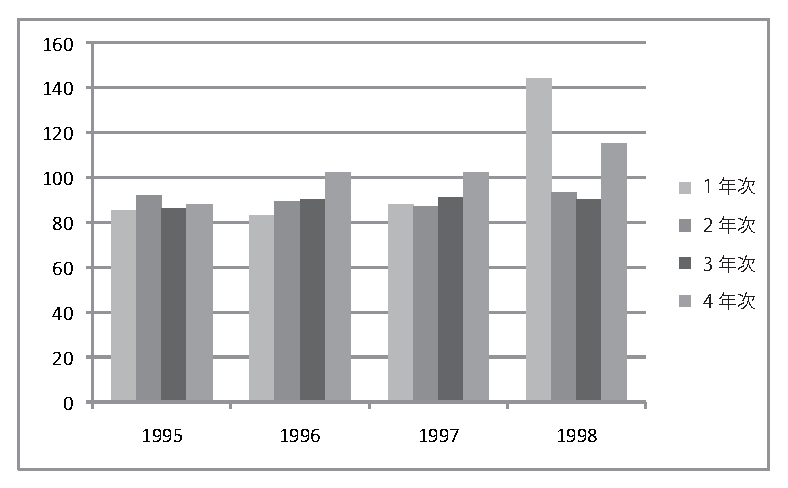
\includegraphics[width=3cm]{sample.eps}
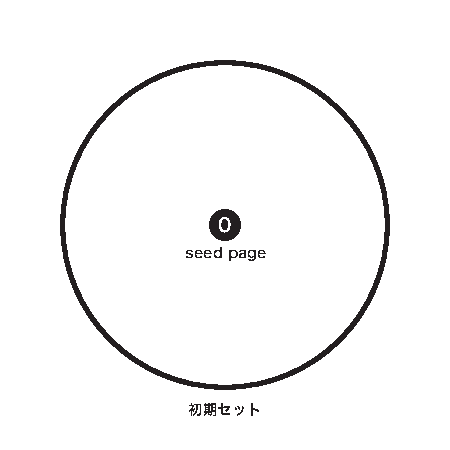
\psfig{file=image/rootset1.eps,scale=1.0}
%\epsfile{file=sample.eps,scale=0.6}
\end{center}
\caption{クラスタへseed pageの追加}
\label{figure:sample}
\end{figure}

\begin{figure}[htbp]
\begin{center}
%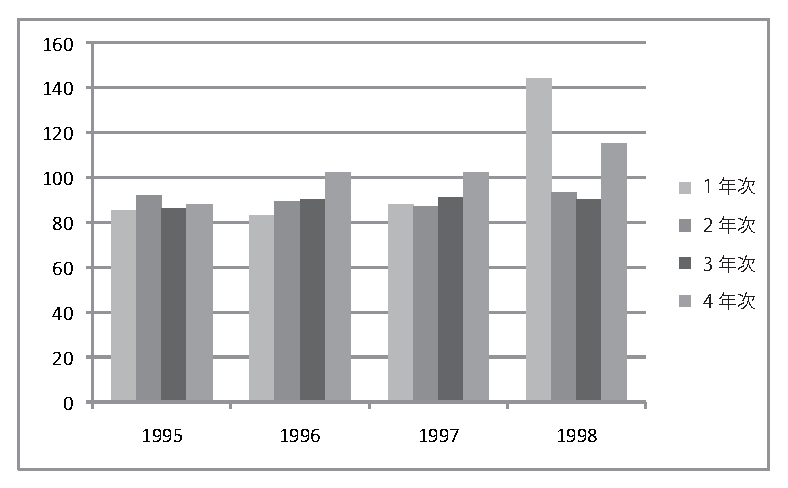
\includegraphics[width=3cm]{sample.eps}
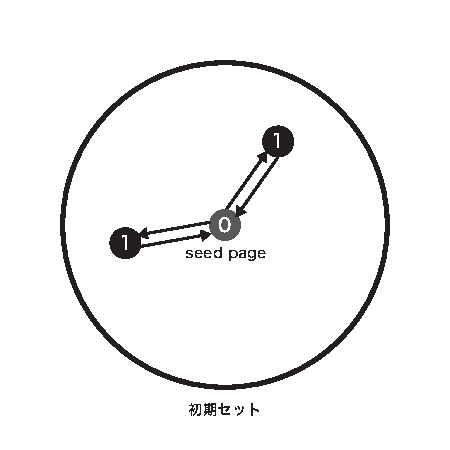
\psfig{file=image/rootset2.eps,scale=1.0}
%\epsfile{file=sample.eps,scale=0.6}
\end{center}
\caption{seed pageと相互リンクしているページの追加}
\label{figure:sample}
\end{figure}

\begin{figure}[htbp]
\begin{center}
%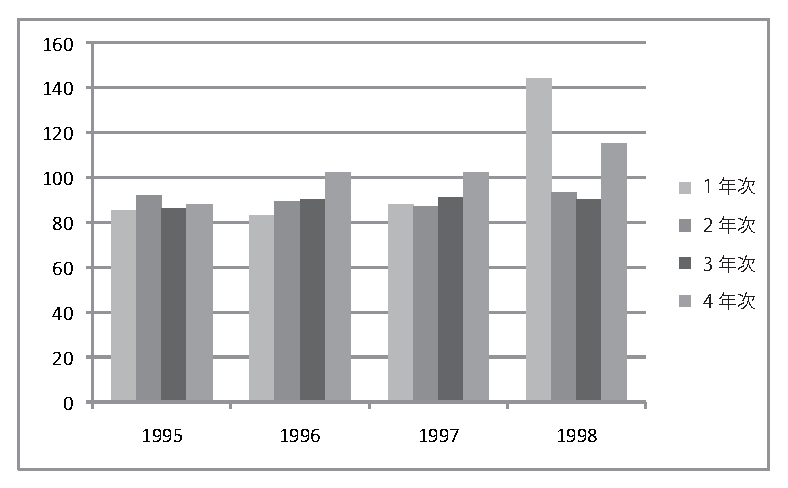
\includegraphics[width=3cm]{sample.eps}
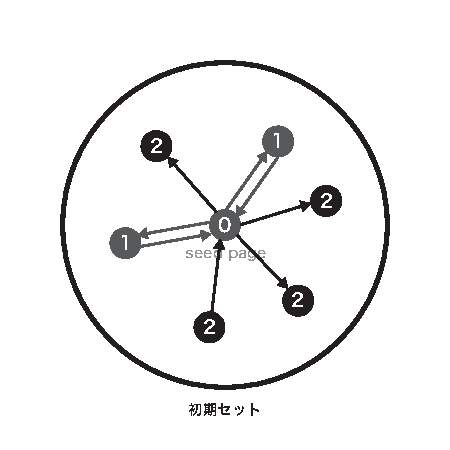
\psfig{file=image/rootset3.eps,scale=1.0}
%\epsfile{file=sample.eps,scale=0.6}
\end{center}
\caption{seed pageの出リンク先、入リンク元であるページの追加}
\label{figure:sample}
\end{figure}

\newpage

先行研究における手法では、初期セットの最大サイズを全ページ数の1/100としていた。
これは、クラスタの最大サイズを全ページ数の約1/10と見積もり、初期セットの最大サイズがさらにその1/10となるように見積もった数値である。この場合、初期セット候補が最大サイズを越えた時、本来seed pageとリンク関係にあるページを適切に抽出することができない。

\begin{figure}[htbp]
\begin{center}
%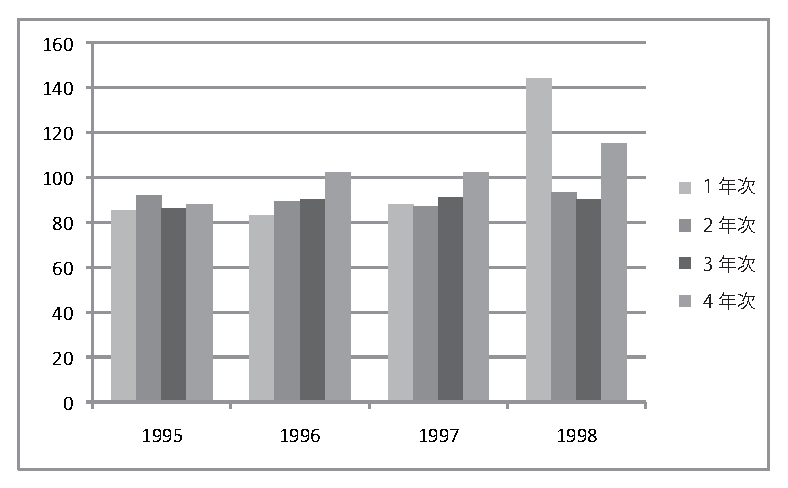
\includegraphics[width=3cm]{sample.eps}

\psfig{file=image/rootset4.eps,scale=1.0}
%\epsfile{file=sample.eps,scale=0.6}
\end{center}
\caption{先行研究における手法での初期セット定義(最大サイズ5とした時)}
\label{figure:sample}
\end{figure}

そこで今回提案する手法では、最終スコアの近似により適したクラスタを作成するため、初期セットのサイズを固定にするのではなく、seed pageとリンク関係にある距離1のページを全て初期セットとする。

\begin{figure}[htbp]
\begin{center}
%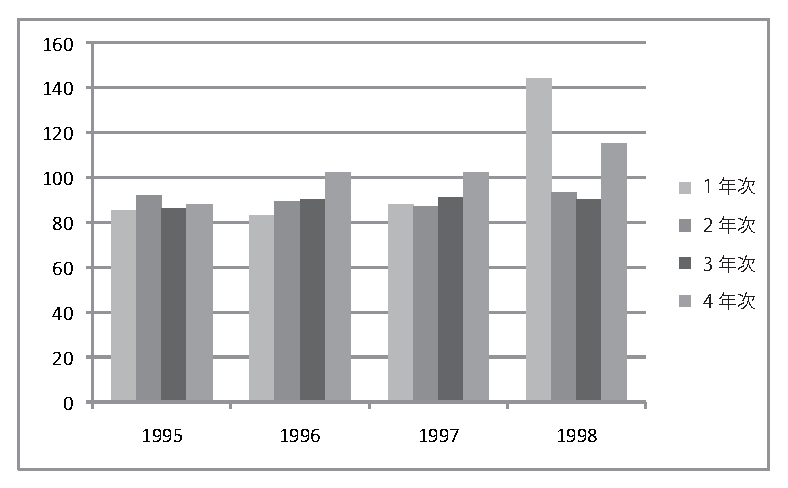
\includegraphics[width=3cm]{sample.eps}
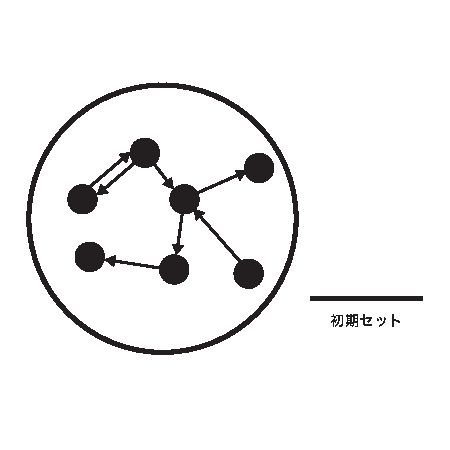
\psfig{file=image/rootset5.eps,scale=1.0}
%\epsfile{file=sample.eps,scale=0.6}
\end{center}
\caption{本研究における手法での初期セット定義}
\label{figure:sample}
\end{figure}

\newpage

初期セットを作成した後は、初期セット内の各ページに対してSALSAスコアを計算し、スコアの高いページとリンクしているページから順にクラスタへ追加していく。

この時、WEBランキングの元となるSALSAスコアの計算上、注意しなければならない点がある。SALSAアルゴリズムでは、各ページの出リンク数と入リンク数によってスコアに重み付けを行う。例えば、ハブスコアの高いページ$i$からリンクされているページ$j$があるとする。このとき、ページ$i$の出リンク数が多い場合、必ずしもページ$j$の権威スコアが高くなるとは限らない。このことから、単純にハブスコアの高いページの出リンク先や、権威スコアの高いページの入リンク元をクラスタに追加することは適切ではない。

そこで、本研究における手法では、クラスタ内での各ページに対して「ハブスコアを出リンク数で割った値」と「権威スコアを入リンク数で割った値」を計算し、それぞれ新たなスコアとする。そこから、新たなハブスコアが高いページの出リンク先と、新たな権威スコアが高いページの入リンク元を、交互にクラスタへ追加することにする。以降、「新たなスコア(元のSALSAスコアを出入リンク数で割った値)が高いページ」のことを「スコアが高いページ」と表現する。

以下の図3.9と3.10でクラスタにページを追加する様子を視覚化した。

\begin{figure}[htbp]
\begin{center}
%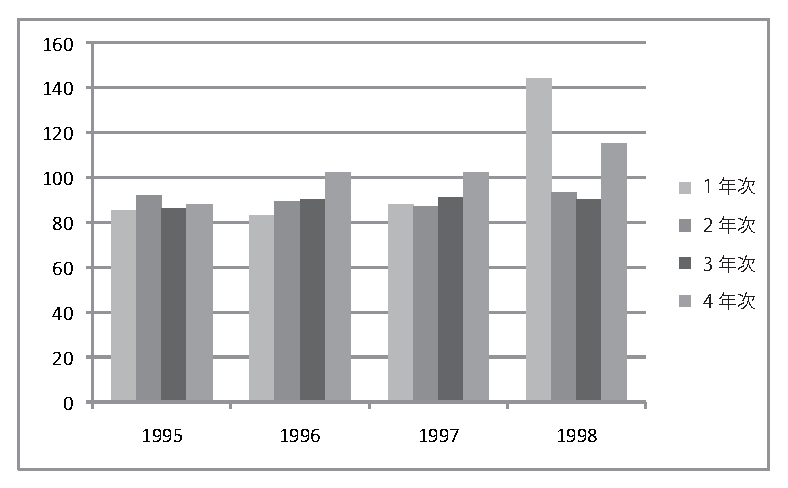
\includegraphics[width=3cm]{sample.eps}
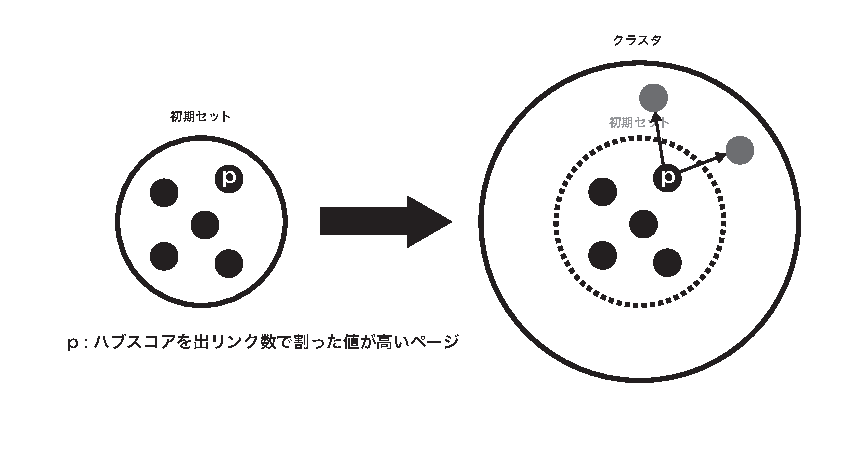
\psfig{file=image/addpage1.eps,scale=1.0}
%\epsfile{file=sample.eps,scale=0.6}
\end{center}
\caption{ハブスコアによるページの追加}
\label{figure:sample}
\end{figure}

\begin{figure}[htbp]
\begin{center}
%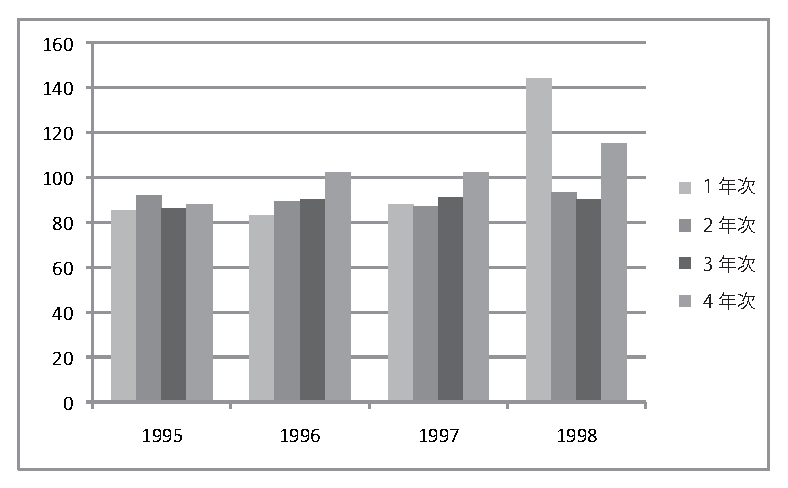
\includegraphics[width=3cm]{sample.eps}
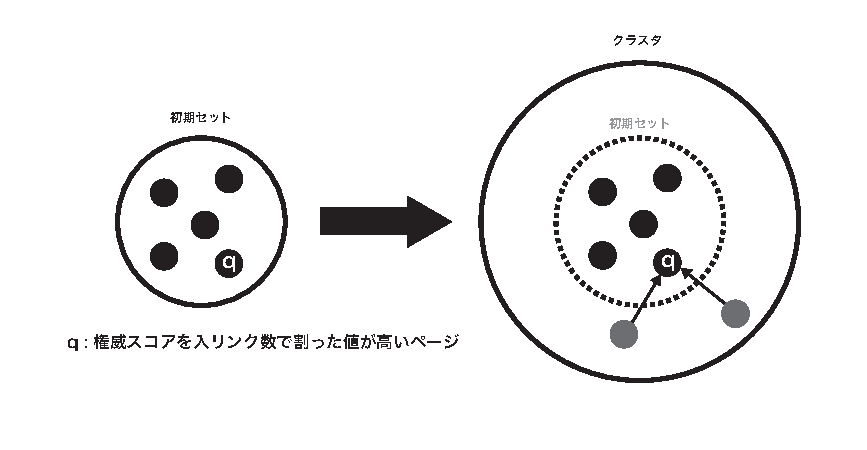
\psfig{file=image/addpage2.eps,scale=1.0}
%\epsfile{file=sample.eps,scale=0.6}
\end{center}
\caption{権威スコアによるページの追加}
\label{figure:sample}
\end{figure}

その後、クラスタ内にあるページの各スコアを基準としてクラスタへのページの追加を終了する。
クラスタにページを追加する際は、前に述べたように、クラスタ内でのスコアが高いページから順にリンクを辿る。ここで、リンクを辿ろうとしているページのスコアがあらかじめ設定した閾値より低くなった時、そのページ以降リンクは辿らずにページの追加を終了する。つまり、新たに追加するページは、まだどのクラスタにも所属せず、かつクラスタ内で閾値より高いスコアを持つページとリンクしている必要がある。この条件を満たすページが存在しなくなった時点でページの追加を終了し、次のクラスタの作成に移る。以下の図3.13 でページの追加を終了する時点でのクラスタの様子を視覚化した。

\begin{figure}[htbp]
\begin{center}
%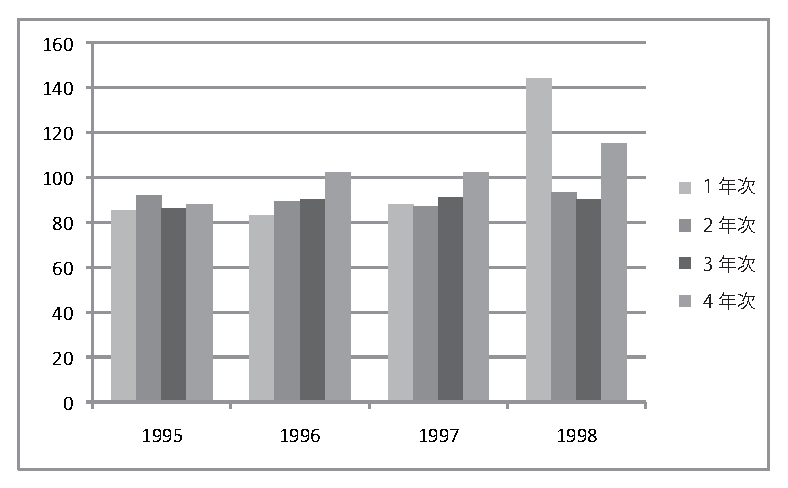
\includegraphics[width=3cm]{sample.eps}
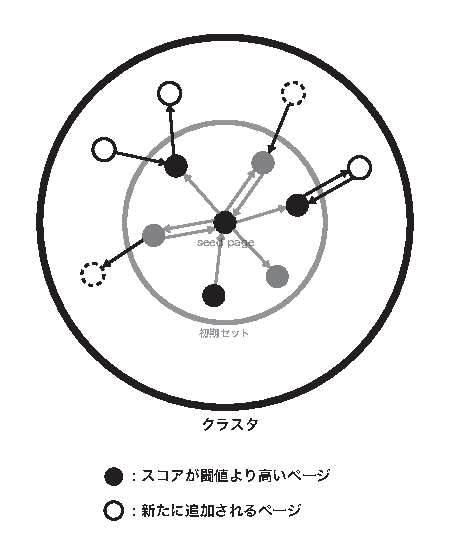
\psfig{file=image/finishclustering.eps,scale=1.0}
%\epsfile{file=sample.eps,scale=0.6}
\end{center}
\caption{ページの追加を終了する時点でのクラスタ}
\label{figure:sample}
\end{figure}

このようにしてクラスタを作成していき、全てのページが1つのクラスタに所属した時点でクラスタリングを全て終了する。

以上のことを踏まえ、クラスタリングアルゴリズムを以下に示す。

\newpage
%%%%クラスタリングアルゴリズム%%%%%%%%%%%%%%%%
\begin{algorithm}
\caption{クラスタリングアルゴリズム}
\begin{algorithmic}[1]

\STATE{PageList = AllPages}
\WHILE{PageList $\neq$ empty}
\STATE{Cluster $<<$ FindSeed}
\STATE{Cluster $<<$ MutualPages(Seed)}
\STATE{Cluster $<<$ InLinkPages(Seed)}
\STATE{Cluster $<<$ OutLinkPages(Seed)}
\STATE{CalcScore(Cluster)}
\LOOP
\IF{TopAuthScorePage.score $>$ 閾値}
\STATE{Cluster $<<$ InLinkPages(TopAuthScorePage)}
\ENDIF
\IF{TopHubScorePage.score $>$ 閾値}
\STATE{Cluster $<<$ OutLinkPages(TopHubScorePage)}
\ENDIF
\IF{TopAuthScorePage.score $<$ 閾値 $\cap$ TopHubScorePage.score $<$ 閾値}
\STATE{break}
\ENDIF
\ENDLOOP
\STATE{ClusterList $<<$ Cluster}
\STATE{PageList = PageList - Cluster}
\ENDWHILE

\end{algorithmic}
\end{algorithm}
%%%%%%%%%%%%%%%%%%%%%%%%%%%%%%%%%%%%

1-2行目は、全てのページがクラスタに所属するまでクラスタリングを続けることを示している。まず1行目で全てのページを記憶したPageListを作成する。1つのクラスタを作成し終わるごとに、20行目でそのクラスタに含まれるページがPageListから削除される。そして、2行目が示しているように、PageListが空になるまでクラスタリングを続ける。

3-6行目ではクラスタの初期セットを作成している。3行目のFindSeed関数でシードとなるページをクラスタへ追加する。ここでシードとなるページは、まだどのクラスタにも所属していない、かつPageListの中で出リンク数や入リンク数の高いものを優先して選ぶ。その後4-5行目で、seed pageと相互リンクしているページをMutualLinkPages関数、seed pageの入リンク元をInLinkPage関数、出リンク先をOutLinkPage関数により取得し、クラスタに追加する。初期セットの作成が完了すると、7行目のCalcScore関数でクラスタ内での各SALSAスコアを計算する。

その後8-18行目を繰り返し、クラスタへページを追加していく。15-17行目が示すように、追加すべきページが存在しなくなるまでクラスタの拡張を続ける。

追加するページを選択するのに、7行目で計算したSALSAスコアを用いる。9-11行目では、権威スコアが閾値より高いページのみ、その入リンク元となるページを追加している。TopAuthSocrePageというのは、初期セット内において権威スコアを入リンク数で割った値が最も高いページであり、.score関数によりその値を取得する。同様に12-14行目では、ハブスコアを出リンク数で割った値が閾値より高いページのみ、その出リンク先となるページを追加している。

これらを繰り返してクラスタの拡張を行う。19行目でClusterListへ保存し、20行目でクラスタに追加したページをPageListから削除している。

\newpage

\section{最終スコアの近似}

最後に、最終スコアの近似方法について解説する。この時点でクラスタリングは終了し、クラスタ内での各ページのスコア計算は終わっているものとする。

クエリが与えられた後、まずクエリと関連するページ(以降クエリページと呼ぶ)が含まれるクラスタを抽出する。その後、それぞれのクラスタに対し、そのクラスタの大きさ、そのクラスタがどれだけクエリページを含んでいるかによって重み付けを行う。これは、クエリとより関連のあるクラスタでのスコアを多く採点するためである。

先行研究におけるクラスタ$c$に対する重み$w_c$を以下の式(3.1)で定義する。

\begin{equation}
w_c = \frac{q}{QN_c}
\end{equation}

ここで、$q$はクラスタ$c$に含まれているクエリページの数であり、$Q$はクエリページの総数である。また、$N_c$はクラスタ$c$の総ページ数である。

本研究における手法では、全てのページは1つのクラスタにのみ所属する。これは先に述べたように、多くのクラスタに所属しているページほどスコアが大きくなることを防ぐためである。それに伴い、最終スコアの近似式にも改良を加える。先行研究では分母に持ってきていたクラスタの総ページ数$N_c$を分子に持ってくる。これによって、クラスタサイズの大きいものほど大きい重みを持つことになる。

本研究におけるクラスタ$c$に対する重み$w_c$を以下の式(3.2)で定義する。

\begin{equation}
w_c = \frac{qN_c}{Q}
\end{equation}

抽出した全てのクラスタに対する重みを計算した後、さらにクエリと関連の高いクラスタの抽出を行う。そして、クエリとの関連が低いクラスタは最終スコアの近似に使用しないこととする。これは、最終スコアの近似計算をするクラスタを減らすことで応答時間を減らすとともに、余計なページをランキングに追加しないためである。

先行研究では、クラスタに対するクエリとの関連度に重みの平均値を用いていた。しかし、平均値を用いる手法では重みに大きくばらつきがあった際に、重みの大きなクラスタのページみがランキングに追加され、重みの小さなクラスタのページはランキングに追加されず、適切なランキングを得ることができなかった。

そこで本研究では、クエリと関連の高いクラスタの抽出に中央値を用いる。中央値とは、測定値を小さい順に並べたとき,ちょうど真ん中にくる値であり、重みの両端に大きな値や小さな値があっても影響されない。また、重みがゼロのものは中央値の計算に考慮しないものとする。重みがゼロのものを除いたクラスタにおける重みの中央値$M_e$は以下の式(3.3)で定義する。

\begin{equation}
M_e =
\begin{cases}
\; X_m & nが奇数のとき,m = (n+1) / 2 \\
\; (X_m + X_{m+1})/2 & nが偶数のとき,m = n/2
\end{cases}
\end{equation}

ここで、$X$は小さい順から並べた各クラスタの重みであり、$n$は重みがゼロのクラスタを除いたクラスタの数である。

次に、抽出したクラスタ内での全てのページに対して近似後の最終スコアを計算する。各ページにおけるスコアは以下の式(3.4)で定義する。

\begin{equation}
score(p,Q) = w_cs(p,c)
\end{equation}

ここで、$Q$はクエリページ集合を表し、$score(p,Q)$はクエリページ集合$Q$に対するページ$p$のスコアを表している。$s(p,c)$はクラスタ$c$におけるページ$p$のスコアである。ここで、$c$は重みが中央値より高いものとする。

以下の図3.14と3.15で最終スコアを近似する流れを視覚化した。図中の円はそれぞれクラスタを表している。

まず、クエリページを含むクラスタを抽出する。図3.14の例ではクラスタa,c,dが該当する。次にそれぞれのクラスタに対する重みをクラスタサイズ、クエリページの総数、クラスタに含まれるクエリページ数から計算する。その結果、重みが中央値以上だったクラスタをa,dとする。ここから、クラスタaとd内の全てのページに対し、近似後の最終スコアを計算する。最後にクエリページを含む全てのクラスタ内の全ページをソートし、ランキングを作成する。

\begin{figure}[htbp]
\begin{center}
%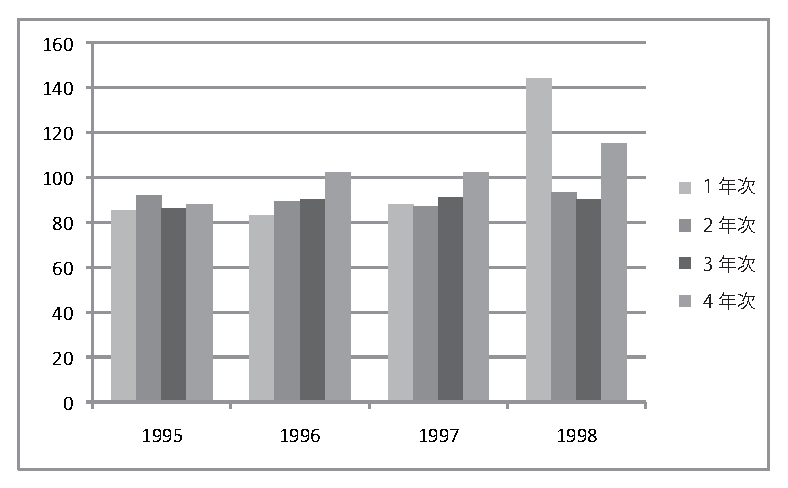
\includegraphics[width=3cm]{sample.eps}
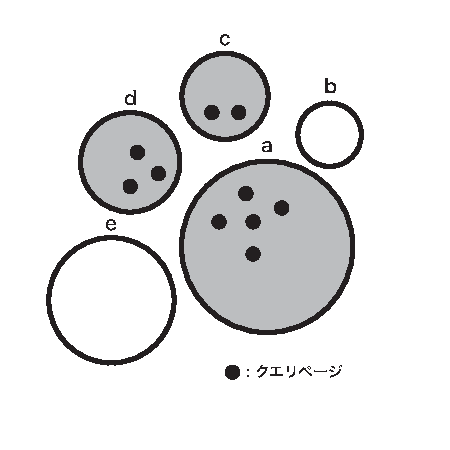
\psfig{file=image/score1.eps,scale=1.0}
%\epsfile{file=sample.eps,scale=0.6}
\end{center}
\caption{クエリページが含まれるクラスタの抽出}
\label{figure:sample}
\end{figure}

\begin{figure}[htbp]
\begin{center}
%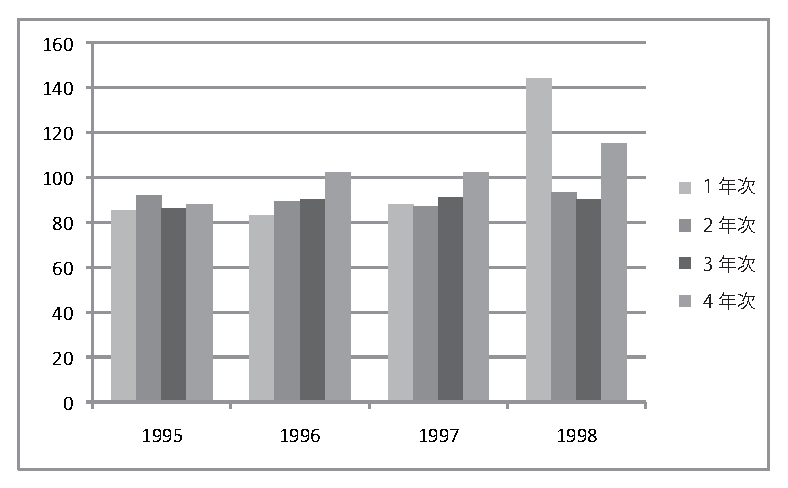
\includegraphics[width=3cm]{sample.eps}
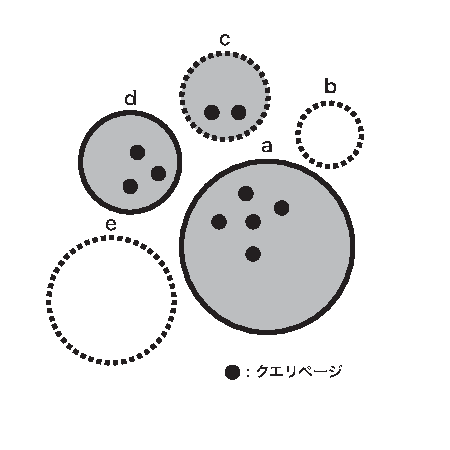
\psfig{file=image/score2.eps,scale=1.0}
%\epsfile{file=sample.eps,scale=0.6}
\end{center}
\caption{重みが中央値以上であるクラスタの抽出}
\label{figure:sample}
\end{figure}

\newpage

以上のことを踏まえ、スコアの近似アルゴリズムを以下に示す。

%%%%最終スコアの近似アルゴリズム%%%%%%%%%%%%%%%%
\begin{algorithm}
\caption{最終スコアの近似アルゴリズム}
\begin{algorithmic}[1]

\STATE{ClusterList = getQueryCluseter(Query)}
\FORALL{Cluster such that Cluster $\in$ ClusterList}
\STATE{Wight $<<$ (HaveQueryNum(Cluster) $*$ Cluster.size) $/$ Query.size}
\ENDFOR
\FORALL{Cluster such that Cluster $\in$ ClusterList}
\IF{Weight[ClusterID] $\geq$ Weight.median}
\STATE{ApproxAuthScore[PageID] = Weight[ClusterID] $*$ Cluster.AuthScore[PageID]} 
\STATE{ApproxHubScore[PageID] = Weight[ClusterID] $*$ Cluster.HubScore[PageID]} 
\ENDIF
\ENDFOR
\end{algorithmic}
\end{algorithm}
%%%%%%%%%%%%%%%%%%%%%%%%%%%%%%%%%%%%

変数Queryは、クエリページの集合である。1行目では、少なくとも1つ以上のクエリページを含むクラスタをgetQueryCluster関数により抽出し、ClusterListを作成している。

2-4行目では、ClusterListの全てのクラスタに対して重みを計算している。3行目のHaveQueryNum関数により、Clusterに所属しているクエリページの数を取得し、クラスタのサイズとかけあわせ、クラスタの総ページ数で割る。計算した重みは中央値の算出と最終スコアの近似に使用するため、配列を使い全て記憶しておく。中央値は.median関数により取得する。

5-9行目で最終スコアの近似を行う。5-6行目が示すように、ClusterListのうち重みが中央値以上であるクラスタのみを用いて計算を行う。7行目では、それぞれのページに対し権威スコアに重みをかけている。8行目では同様にハブスコアに重みをかけている。Cluster.AuthScoreおよびCluster.HubScoreは、それぞれ書くページにおけるクラスタ内での権威スコアとハブスコアである。ApproxAuthScoreおよぶApproxHubScoreは、それぞれ各ページにおける最終的な権威スコアとハブスコアである。

最後に、近似された最終スコアをソートすることでランキングを作成し、掲示する。

%%%%%%%%%%%%%%%%%%%%%%%%%%%%%%%%%%%%%%%%%%%%%%%%
\chapter{実験と考察}

\section{評価指標}

従来のSALSAアルゴリズムと提案手法を用いて、同一のWEBページの集合から2つのWEBランキングを作成し比較する。従来のSALSAアルゴリズムで作成されたWEBランキングと、提案手法によって作成されたWEBランキング、どれだけ一致しているかについての評価指標として適合率を用いた。

適合率は以下の式(4.1)で表すことができる。

\begin{equation}
presicion = \frac{R}{N}
\end{equation}

ここでRは、一方のWEBランキングに含まれるページの内、もう一方のWEBランキングにも含まれているページの数である。Nはランキングのサイズである。適合率は、2つのランキングがどれほどランキング内に同じページを含んでいるかを表し、0から1までの値を取る。2つのランキングが全て同じページの場合で最大の1を、同じページが全く含まれていない場合で最小の0を返す。

また、従来のSALSAアルゴリズムと提案手法の応答速度の比較は以下の式(4.2)で定義する。

\begin{equation}
response = \frac{q}{p} \times 100
\end{equation}

ここでpは従来のSALSAアルゴリズムにおける応答時間であり、qは前処理を行った高速化SALSAアルゴリズムの応答時間である。従来のSALSAアルゴリズムの応答時間を100$\%$とした時、提案手法の応答時間がどれだけ短くなっているかを表している。

\section{実データでの実験}
\section{大規模データでの実験}

%%%%%%%%%%%%%%%%%%%%%%%%%%%%%%%%%%%%%%%%%%%%%%%%
\chapter{まとめ}

てすてす

%%%%%%%%%%%%%%%%%%%%%%%%%%%%%%%%%%%%%%%%%%%%%%%%
\chapter{形式}

ここでは、論文の表紙および本体の記述方法について述べる。

\section{表紙}

表紙は、{\tt $\backslash$maketitle} によって作成するため、以下の項目に相
当する文字列をそれぞれ記述する。

\begin{description} \parskip=1pt
\item{題目: }
題目は{\tt $\backslash$title} に記述する。行替えを行う場合は$\backslash$
	   $\backslash$ を入力する。ただし、題目の最後に$\backslash$
	   $\backslash$ を入力するとコンパイルが通らなくなるので注意する。
	   なお、4行以上の題目の場合、表紙ページがあふれるためスタイルファ
	   イル``mast-jp-sjis.sty''を変更する必要がある。
\item{著者名: }
著者名は{\tt $\backslash$author} に記述する。
\item{指導教員名: }
指導教教員は{\tt $\backslash$advisor} に記述する。
\item{年月: }
年月は{\tt $\backslash$yearandmonth} に記述する。年月は提出時のものを記述すること。
\end{description}

\section{本体}

本体は1段組で記述する。

図表には番号と説明(caption)を付け、文章中で参照する。表
\ref{table:fundamental_data_type}と図\ref{figure:sample}はそれぞれ表と図
の例である。表の説明は上に、図の説明は下に書くことが多い。図の挿入に用い
るパッケージについては使用環境に合わせて自由に選択してほしい。

\begin{table}[hbt]
\caption{表の例}
\label{table:fundamental_data_type}
\begin{center}
\begin{tabular}{| c | r | r | r | r |}
\hline
年 度 & 1年次 & 2年次 & 3年次 & 4年次 \\
\hline
1995 & 85 & 92 & 86 & 88 \\
1996 & 83 & 89 & 90 & 102 \\
1997 & 88 & 87 & 91 & 112 \\
1998 & 144 & 93 & 90 & 115 \\
\hline 
\end{tabular}
\end{center}
\end{table}
\medskip


詳しくは参考書\cite{okumura2010,yoshinaga2009}などを参照のこと。
また、奥村晴彦氏の「\TeX Wiki」
http://oku.edu.mie-u.ac.jp/\textasciitilde{}okumura/texwiki/
は、日本語の\TeX に関する情報が充実している。
また、具体的な論文としての文献参照例として
(本の例)\cite{ware2004}、
(雑誌論文の例)\cite{meyer2009}、
(予稿集の例)\cite{hill2010}
を挙げておく。

\chapter*{謝辞}
\addcontentsline{toc}{chapter}{\numberline{}謝辞}

感謝

\newpage


\addcontentsline{toc}{chapter}{\numberline{}参考文献}
\renewcommand{\bibname}{参考文献}

%% 参考文献に jbibtex を使う場合
%\bibliographystyle{junsrt}
%\bibliography{samplebib}
%% [compile] jbibtex sample; platex sample; platex sample;

%% 参考文献を直接ファイルに含めて書く場合
\begin{thebibliography}{1}
\bibitem{okumura2010}
奥村晴彦, LaTeX2e美文書作成入門 改訂第5版, 技術評論社, 2010年.

\bibitem{yoshinaga2009}
吉永徹美, LaTeX2ε辞典, 翔泳社, 2009年.

\bibitem{ware2004} 
Colin Ware, Information Visualization --- Perception for Design, Second Edition, Morgan Kaufmann Publishers, 486~p., 2004.

\bibitem{meyer2009}
Miriah Meyer and Tamara Munzner, MizBee: A Multiscale Synteny Browser, {\em IEEE Transactions on Visualization and Computer Graphics}, Vol.~15, No.~6, pp.~897--904, 2009.

\bibitem{hill2010}
Emerson Murphy-Hill and Andrew P. Plack, An Interactive Ambient Visualization for Code Smells, {\em in Proceedings of the 2010 International Symposium on Software Visualization (SOFTVIS’10)}, pp.~5--14, 2010.

\end{thebibliography}




\end{document}
